% Session 2 -- three archetypes of dispersion and the density of states each produces.
% Placement: sec. "Three archetypes of dispersion", alongside the enumerated list.
% Rendered by figures/blender/s02f06_archetypes.py, labels in figures/overlays/s02f06_archetypes.tex.
\begin{aqmfigure}{fig:s02:archetypes}{The three types of dispersion and the densities of states that
they give, all in \emph{two} dimensions. Each band is a surface over the two-dimensional momentum,
with its density of states as a slab next to it on the same energy axis. A parabolic band gives a
constant density of states, which is a step. A Dirac point makes it vanish linearly, so a finite
interaction strength is needed before anything happens. A flat band makes it diverge, drawn here
with a small broadening, so an arbitrarily weak interaction can drive the symmetry-broken states of
Session 1. Almost every band structure in this course is locally one of these three.}
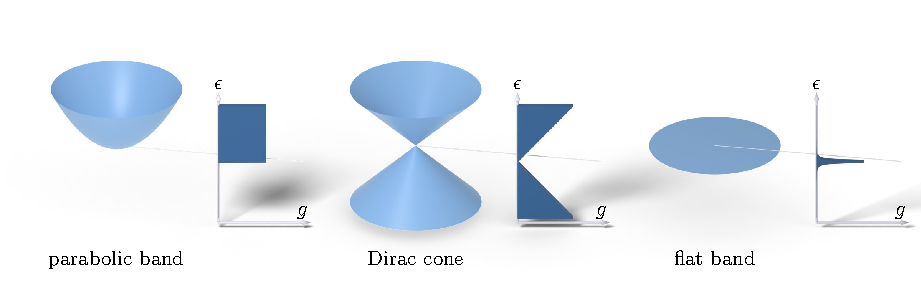
\includegraphics{figures/pdf/s02f06_archetypes.pdf}
\end{aqmfigure}
